
%% SC 2014
%% Poster text
%% http://sc14.supercomputing.org/program/posters
%% Due: August 7, 2014
%% Page limit: 2

\documentclass[conference,10pt]{IEEEtran}
%\usepackage{epsfig}
\usepackage{amssymb}
\usepackage{amsmath}
\usepackage{amsfonts}
%\usepackage{backnaur}
%\usepackage{clrscode3e}
\usepackage[T1]{fontenc} % get tt fonts to work right
\usepackage{graphicx}
\usepackage{multirow}
\usepackage{color}
\usepackage{comment}
\usepackage{caption}
\DeclareCaptionType{copyrightbox} % workaround for bug in caption
\usepackage{subcaption}
\usepackage{tikz}
%\usepackage{paralist}
\usepackage{xspace}
%\usepackage{numprint} % print numbers with thousands separator

% A definition we do not want the reader to forget
%\newcommand{\defn}[1] {\textbf{\textit{#1}}}
\newcommand{\defn}[1] {\textit{#1}}

\newcommand{\SwiftT}{Swift/T\xspace}
\newcommand{\STC}{STC\xspace}

\newcommand*\circled[1]{\tikz[baseline=(char.base)]{
  \node[shape=circle,draw,inner sep=2pt] (char) {#1};}}


% Symbols used to represent congruence
\newcommand{\valcong}{\cong^V}
\newcommand{\aliascong}{\cong^A}

\definecolor{darkblue}{rgb}{0,0,0.7}
\definecolor{darkgreen}{rgb}{0,0.5,0}
\definecolor{orange}{rgb}{0.7,0.5,0.0}
\definecolor{brown}{rgb}{0.8,0.4,0.0}

\definecolor{teal}{rgb}{0.06,0.3,0.3}
\definecolor{maroon}{rgb}{0.5,0.0,0.25}
\definecolor{darkblue}{rgb}{0.0,0.2,0.75}
\definecolor{darkred}{rgb}{0.7,0.0,0.0}
\definecolor{darkgreen2}{rgb}{0,0.35,0}
\definecolor{darkgreen}{rgb}{0,0.5,0}

\newif\ifdraft
%\drafttrue
\draftfalse
\ifdraft
  \newcommand{\woz}[1]{ {\textcolor{darkgreen} { Wozniak: #1 }}}
  \newcommand{\arm}[1]{ {\textcolor{darkred} { Tim: #1 }}}
  \newcommand{\katznote}[1]{ {\textcolor{darkblue} { Dan: #1 }}}
  \newcommand{\mw}[1]{ {\textcolor{blue} { Mike: #1 }}}
  \newcommand{\ian}[1]{{\textcolor{red}{ Ian: #1}}}
\else
 \newcommand{\woz}[1]{}
 \newcommand{\arm}[1]{}
\fi

\definecolor{swiftbuiltincolor}{rgb}{0,0,0}
\definecolor{swiftstringcolor}{rgb}{0,0,0}
\definecolor{swiftcommentcolor}{rgb}{0,0,0}

\hyphenation{foreach}
\hyphenation{work-stealing}


% Space management
\addtolength{\textfloatsep}{-1em}
\addtolength{\dbltextfloatsep}{-1em}
\addtolength{\abovecaptionskip}{-.5em}
\addtolength{\belowcaptionskip}{-.75em}
\linespread{1}

\newenvironment{tightitem}%
  {\begin{itemize}%
    \addtolength{\topsep}{0em}%
    \addtolength{\parsep}{0em}%
    \addtolength{\itemsep}{0em}%
    \addtolength{\parskip}{-0.25em}}%
  {\end{itemize}}

\begin{document}

\special{papersize=8.5in,11in}
\setlength{\pdfpageheight}{\paperheight}
\setlength{\pdfpagewidth}{\paperwidth}

\newcommand{\topic}[1] { { \noindent $\bullet$ \textbf{ #1:}}}


\title{Discovery Engines: Connecting X-ray Experiments to HPC Analysis}

\author{\IEEEauthorblockN{
Justin M. Wozniak,\IEEEauthorrefmark{1}\IEEEauthorrefmark{2}
Hemant Sharma,\IEEEauthorrefmark{1}
Michael Wilde,\IEEEauthorrefmark{1}\IEEEauthorrefmark{2}
Ian T. Foster\IEEEauthorrefmark{1}\IEEEauthorrefmark{2}\IEEEauthorrefmark{3}}
  \IEEEauthorblockA{
  \IEEEauthorblockA{\IEEEauthorrefmark{1}Mathematics and Computer Science Division,
    Argonne National Laboratory,
    Argonne, IL, USA}
  \IEEEauthorblockA{\IEEEauthorrefmark{2}Computation Institute,
    University of Chicago and Argonne National Laboratory,
    Chicago, IL, USA}
  \IEEEauthorrefmark{3}Dept. of Computer Science,
    University of Chicago,
    Chicago, IL, USA}
}

\maketitle

\section{Overview}

High-energy diffraction microscopy (HEDM) is an important method for
determining the grain structure of metals.  It is performed at
specialized light sources such as the Advanced Photon Source (APS) at
Argonne National Laboratory (ANL).  In the typical scientific
workflow, the scientist applies for a week of beam time and spends
that time gathering data.  Over the next several months, the data is
processed using custom-built tools.  High-performance computing (HPC)
is rarely if ever applied during the week of beam time.  Applying HPC
to quickly analyze the data produced by the experiment detectors has
the potential to greatly reduce errors.  It may provide feedback to
the scientist during the run, to improve the quality of results and
the utility of precious beam time.  Most importantly, it will speed
the process of scientific discovery, even if the HPC is applied after
beam time. In this work, we present an HEDM application that spans a
small cluster and the Blue Gene/Q at ANL.  It uses up to 64K cores of
the BG/Q to provide near real-time feedback to APS beam users.

\section{High-energy diffraction microscopy at the APS}

APS beamline scientists H. Sharma and J. Almer, performing experiments
at APS Sector 1-ID, are developing new experimental techniques and
algorithms for determining the grain structure of polycrystalline
material samples, via high-energy diffraction microscopy (HEDM).  In
close collaboration with DEBD, they are applying new tools and methods
to parallelize (and dramatically speed up) their new algorithms;
enhance them with data and metadata management techniques; and make
them available to the broader APS and scattering communities.

\subsection{Scientific overview}

HEDM is used to non-destructively determine the grain structure of
polycrystalline materials. It's a valuable technique for the analysis of
grain defects in advanced alloy materials, such as those used in
turbine blades for both energy (e.g. wind turbines) and engine
applications (e.g. jet engine turbines). The technique allows a
material sample, or even a manufactured part, to be studied within an
APS beamline across a dynamically varying range of concurrent thermal
and tensile stresses.  A polycrystalline material sample (typically a
metal alloy) is positioned in the X-ray beam, and the diffraction
pattern of the beam as it passes through the sample is collected by a
detector.  The diffraction patterns are then analyzed by software
tools to reconstruct the granular structure of the material, with a
focus on determining the granular structure of material defects that
can cause component failure in fabricated parts.

A line-focus X-ray beam is used to collect diffraction data from
a 2D cross-section (``layer'') of a rotating polycrystalline sample
using a high-resolution detector (1.5 micron pixel size) placed in close
proximity to the sample (less than 10 mm away). 2D TIFF format images, 8MB in
size, are collected from the detector. At each angle of rotation,
typically 360 to 1440 angles per layer, 8MB per file, are stored on
the s1idserv file server. A new layer (3 to 12 GB of raw data) is
collected every 3-5 minutes. As in the case of FF-HEDM, the
acquisition is performed using a set of ``SPEC'' scripts. The metadata
of each layer is stored in a separate file.

\subsection{Workflow details}

The raw TIFF files are reduced to binary files containing only
information about the diffraction signal of the detector. Due to the
sparse nature of the data, each 8 MB raw file can be reduced to a
binary file of about 1 MB. This reduction is performed using 320 CPUs
on Orthros, each using about 2 min of CPU time. These binary files are
fed into an orientation detection program to map the orientation of
each point in a grid in the 2D cross-section of the sample. Two
approaches are possible for this step.  Using 320 CPUs on Orthros, at
about 30s for each grid point (a total of 100k grid points), we can
obtain results in 3 hours.  Using 10,000 CPUs on the Mira BG/Q or a
similarly parallel resource, we can scale this workflow to obtain
results in less than 5 min.

The output is a text or binary file (selectable by the user), about 10
MB in size, containing information about the orientation of each point
in a grid in the 2D cross-section of the sample.  All analysis
software has been developed in-house in Sector 1, implemented in
C. Parallel processing of the analysis routines is implemented using
the Swift parallel scripting language in collaboration with the DEBD
project.

\begin{figure}
  \begin{center}
    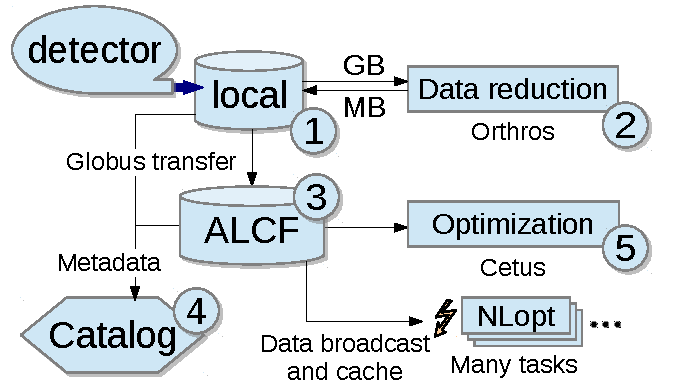
\includegraphics[scale=0.58,clip=true,trim=0.05in -0.3in 0 0]
                    {img/NFHEDM.pdf}
    \caption{Cross-lab APS to ALCF workflow.
      \label{figure:nfhedm-workflow}}
  \end{center}
\end{figure}

A detailed diagram of the workflow for NF-HEDM is shown in
Figure~\ref{figure:nfhedm-workflow}.  In this figure, the detector
produces data on an NFS installation at the APS~\circled{1}. A large
batch of data reduction jobs are run on the local cluster, named
Orthros~\circled{2}.  The data is moved via Globus to Argonne
Leadership Computing Facility (ALCF) storage~\circled{3}, and stored
in a metadata catalog~\circled{4}~\cite{Catalog_2014}.  Finally, the
HPC component begins~\circled{5}- a large batch of hundreds of
thousands of optimization operations are performed rapidly across tens
of thousands of CPU cores of a Blue Gene/Q.

\section{Many-task parallelization for HEDM}



The HPC component of the workflow was implemented using
Swift/T~\cite{SwiftT_2013}, a dataflow programming system implemented
atop the Turbine runtime~\cite{Turbine_2013} and the Asynchronous
Dynamic Load Balancer~\cite{ADLB_2010}.  In this model, C analysis
code developed for this work is linked to the NLopt optimizer library
and the GNU scientific library.  These C code tasks are grouped into a
large Swift script, which compiles into an MPI program for execution
on a large HPC resource.  Swift/T has been shown to scale to over a
billion tasks/second on hundreds of thousands of cores~\cite{STC_2014}
or GPUs~\cite{Krieder_2014}.




\section{Performance} 

\begin{figure}
  \begin{center}
    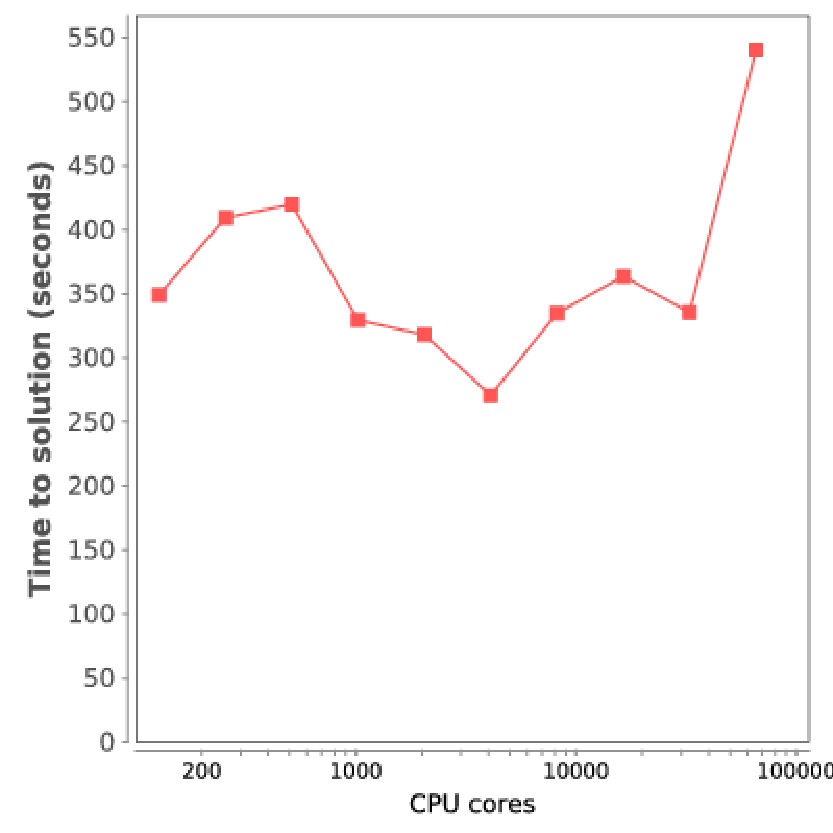
\includegraphics[scale=0.58,clip=true,trim=0.05in -0.3in 0 0]
                    {plots/nf-hedm.pdf}
    \caption{Cross-lab APS to ALCF workflow.
      \label{figure:nfhedm-workflow}}
  \end{center}
\end{figure}

To measure performance of the HPC portion of the workflow, we ran it
on several allocation sizes of the Blue Gene/Q systems at ANL.  In
each run, only one task is processed by each processor.  This emulates
the case in which the scientist has access all available cores, and
desires the fastest result.  The time to solution is limited by the
slowest task- task runtimes may vary as the optimization routine is
not easily predictable.  

Our implementation performs well up to 32K cores, after which some
slowdown is observed.  Performance is dependent on input rates, as the
whole dataset must be read by each process.  Thus, run times vary
widely due  to other users of the filesystem.  At 64K cores,
performance drops a bit, probably due to I/O, which will be the focus
of our future work.  

\section{Summary}

This work presented the initial application of HPC to an X-ray HEDM
problem, and showed that HPC can solve the whole analysis phase of the
workflow extremely quickly ($\sim$ 5 minutes).  Future work will
refine the workflow and improve the use of I/O to achieve better
performance on the maximal required number of cores. 

\section*{Acknowledgments}

This research is supported by the U.S. DOE Office of Science under
contract DE-AC02-06CH11357 and NSF award ACI 1148443.  Computing
resources were provided in part by NIH through the Computation
Institute and the Biological Sciences Division of the University of
Chicago and Argonne National Laboratory, under grant S10 RR029030-01,
and by NSF award ACI 1238993 and the state of Illinois through the
Blue Waters sustained-petascale computing project. This research used
resources of the Argonne Leadership Computing Facility at Argonne
National Laboratory, which is supported by the Office of Science of
the U.S. Department of Energy under contract DE-AC02-06CH11357.

\bibliographystyle{abbrv}
\bibliography{swift}

\begin{comment}

\vspace{1cm}

\noindent
(The following paragraph will be removed from the final version.)

\vspace{0.5cm}

\noindent
This manuscript was created by UChicago Argonne, LLC, Operator of
Argonne National Laboratory (``Argonne''). Argonne, a U.S. Department
of Energy Office of Science laboratory, is operated under Contract
DE-AC02-06CH11357.  The U.S. Government retains for itself, and others
acting on its behalf, a paid-up nonexclusive, irrevocable worldwide
license in said article to reproduce, prepare derivative works,
distribute copies to the public, and perform publicly and display
publicly, by or on behalf of the Government.

\end{comment}

\end{document}
